%
% File acl2014.tex
%
% Contact: koller@ling.uni-potsdam.de, yusuke@nii.ac.jp
%%
%% Based on the style files for ACL-2013, which were, in turn,
%% Based on the style files for ACL-2012, which were, in turn,
%% based on the style files for ACL-2011, which were, in turn, 
%% based on the style files for ACL-2010, which were, in turn, 
%% based on the style files for ACL-IJCNLP-2009, which were, in turn,
%% based on the style files for EACL-2009 and IJCNLP-2008...

%% Based on the style files for EACL 2006 by 
%%e.agirre@ehu.es or Sergi.Balari@uab.es
%% and that of ACL 08 by Joakim Nivre and Noah Smith

\documentclass[11pt]{article}
\usepackage{acl2014}
\usepackage{times}
\usepackage{url}
\usepackage{latexsym}
\usepackage[backend=bibtex]{biblatex}
\usepackage{graphicx}
\addbibresource{citations}


%\setlength\titlebox{5cm}

% You can expand the titlebox if you need extra space
% to show all the authors. Please do not make the titlebox
% smaller than 5cm (the original size); we will check this
% in the camera-ready version and ask you to change it back.


\title{MIM QA System: Deliverable 2}

\author{Antariksh Bothale \\
  {\tt abothale@uw.edu} \\\And
  Julian Chan\\
  {\tt jchan3@uw.edu} \\\And
  Yi-shu Wei\\
  {\tt yishuwei@uw.edu}}

\date{}

\begin{document}
\maketitle
\begin{abstract}
We introduce the preliminary work done on MIM, our Question Answering system.
\end{abstract}

\section{Introduction}
This document reports the creation and performance of an end-to-end Question Answering system. We have a basic setup in place for the overall task and present current baseline results.  

\section{System Overview}

Our system architecture can be broken down into three major classes - MainFacilitator, TaskExecutor, and Session. Our information retrieval system processes queries and retrieves answers in 3 steps, namely Document Retrieval, Passage Retrieval, and Answer Processing. Each of these steps are encapsulated in their own class and derives from the TaskExecutor task.  The Session object is used to pass information between these tasks. The implementation of each TaskExecutor is completely transparent to the MainFacilitator, whose job is to simply run the TaskExecutor(s) in the correct order and pass a Session object between them. The QuestionProcessor object is embedded in the Session object and contains methods that allows the TaskExecutor(s) to access the user query.

During start-up, MainFacilitator instantiates the three TaskExecutor(s) and put them in an array. When there is a new query and the AnswerQuestion() method is called, MainFacilitator creates a new Session object and calls Execute() on each of the TaskExecutor(s) sequentially. Barring any execution error, the answer will be written to the Session object. 

The SystemEvaluator reads in all the question from the data set and calls MainFacilitator's AnswerQuestion() function. It then reads the answer from the returned Session object and 
writes to the output file.

%\begin{figure*}
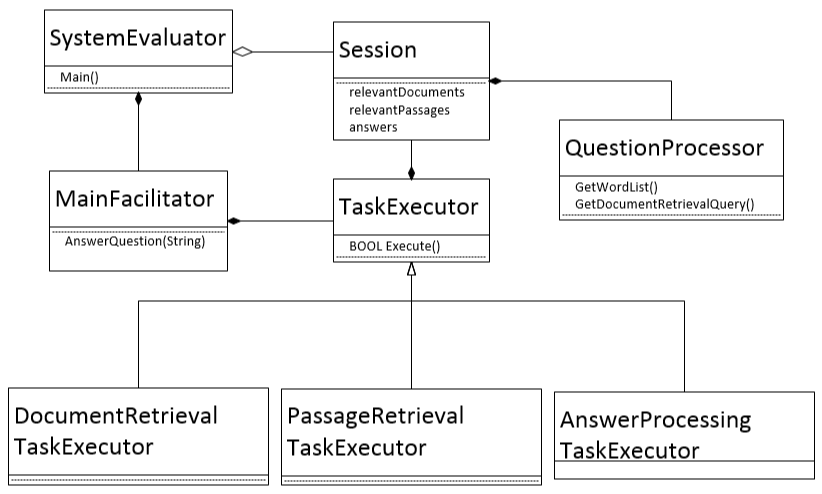
\includegraphics[width=3in,height=1.75in]{MIM_class_diagram.png}
Fig 1: class diagram of the MIM QA system
%\end{figure*}


\section{Approach}
\subsection{Document Retrieval}
The Document Retrieval Subsystem takes a document retrieval query from the session and populates the session with a list of hits from the indexing and retrieval system, as described below. This list of documents is then used for Passage Retrieval and Answer Processing.

For the purpose of indexing and searching the documents, we use Whoosh\cite{whoosh}, which is pure-Python based text indexing, search, and spell checking library. The choice of a Python based library above alternatives such as Lucene and Indri/Lemur was motivated by its ease of integration and use with our Python code-base, and its functionality being comparable to that of its Java counterparts. 

\subsubsection{Indexing}
The Beautiful Soup XML parser\cite{bsoup} was used to parse all the documents and extract the Document ID, Headline and Body Text. Whoosh's in-built indexing engine was used to index all the documents present in the corpus. The current system uses Whoosh's default indexing mechanism, which does not process the text, we plan to improve on this by incorporating tokenization and stemming. The indexing schema was designed to store the Document ID and Headline with the Index, while the Body Text was indexed but not stored as it would have caused unnecessary duplication of data. Instead, the text is retrieved from the document using the Document ID whenever needed. This index is currently stored on Patas.

\subsection{Passage Retrival and Answer Extration}
In this deliverable we combine passage retrieval and answer extraction into one step. This step reads the files reported as relevant by the document retrieval module, extracting all passages in the documents that contain the keywords (the words in the question). A ``passage'' in our current system is simply defined as any chunk within the document with no more than 250 characters. These passages are than scored based on the density of keywords in the passage. The passage extraction and scoring function are taken from Whoosh, which are originally used for returning snippets for search results. The final answers of our current system are the top three passages.

In the future version of our system, we would like to split out an separate answer extraction modeule so that it will generate short answers from the passages and score them based on whether they are valid answers to the question type and their relevance. We would also like to improve the passage retrieval part by implementing our own passage scoring function.

\section{Results}

Under the baseline system, we obtain an aggregate score of 0.0466 under the Strict evaluation scheme, and an aggregate score of 0.0595 under the Lenient evaluation scheme.
One reason we got such low scores is that we did not notice there is an \texttt{text} attribute in the parent node of the questions (the \texttt{target} node) which contains the main subject of the questions. Our search was based on the question text only, and thus missed the most important information.

\section{Discussion}
\label{sec:discussion}

The baseline system has been put in place and works end to end, but since it uses fairly naive and rudimentary processing methods at each step of the chain, the results are far from satisfactory. The next few weeks on the project would now be devoted to improving each of the segments. 
\section*{Acknowledgments}


\printbibliography 

\end{document}
